\documentclass[journal,12pt,twocolumn]{IEEEtran}
%
\usepackage{setspace}
\usepackage{gensymb}
%\doublespacing
\singlespacing

%\usepackage{graphicx}
%\usepackage{amssymb}
%\usepackage{relsize}
\usepackage[cmex10]{amsmath}
\usepackage{siunitx}
%\usepackage{amsthm}
%\interdisplaylinepenalty=2500
%\savesymbol{iint}
%\usepackage{txfonts}
%\restoresymbol{TXF}{iint}
%\usepackage{wasysym}
\usepackage{amsthm}
\usepackage{iithtlc}
\usepackage{mathrsfs}
\usepackage{txfonts}
\usepackage{stfloats}
\usepackage{steinmetz}
%\usepackage{bm}
\usepackage{cite}
\usepackage{cases}
\usepackage{subfig}
%\usepackage{xtab}
\usepackage{longtable}
\usepackage{multirow}
%\usepackage{algorithm}
%\usepackage{algpseudocode}
\usepackage{enumitem}
\usepackage{mathtools}
\usepackage{tikz}
\usepackage{circuitikz}
\usepackage{pgfplots}
\usepackage{verbatim}
\usepackage{tfrupee}
\usepackage[breaklinks=true]{hyperref}
%\usepackage{stmaryrd}
\usepackage{tkz-euclide} % loads  TikZ and tkz-base
%\usetkzobj{all}
\usetikzlibrary{calc,math}
\usetikzlibrary{fadings}
\usepackage{listings}
    \usepackage{color}                                            %%
    \usepackage{array}                                            %%
    \usepackage{longtable}                                        %%
    \usepackage{calc}                                             %%
    \usepackage{multirow}                                         %%
    \usepackage{hhline}                                           %%
    \usepackage{ifthen}                                           %%
  %optionally (for landscape tables embedded in another document): %%
    \usepackage{lscape}     
\usepackage{multicol}
\usepackage{chngcntr}
%\usepackage{enumerate}

%\usepackage{wasysym}
%\newcounter{MYtempeqncnt}
\DeclareMathOperator*{\Res}{Res}
%\renewcommand{\baselinestretch}{2}
\renewcommand\thesection{\arabic{section}}
\renewcommand\thesubsection{\thesection.\arabic{subsection}}
\renewcommand\thesubsubsection{\thesubsection.\arabic{subsubsection}}

\renewcommand\thesectiondis{\arabic{section}}
\renewcommand\thesubsectiondis{\thesectiondis.\arabic{subsection}}
\renewcommand\thesubsubsectiondis{\thesubsectiondis.\arabic{subsubsection}}

% correct bad hyphenation here
\hyphenation{op-tical net-works semi-conduc-tor}
\def\inputGnumericTable{}                                 %%

\lstset{
%language=C,
frame=single, 
breaklines=true,
columns=fullflexible
}
%\lstset{
%language=tex,
%frame=single, 
%breaklines=true
%}

\begin{document}
%


\newtheorem{theorem}{Theorem}[section]
\newtheorem{problem}{Problem}
\newtheorem{proposition}{Proposition}[section]
\newtheorem{lemma}{Lemma}[section]
\newtheorem{corollary}[theorem]{Corollary}
\newtheorem{example}{Example}[section]
\newtheorem{definition}[problem]{Definition}
%\newtheorem{thm}{Theorem}[section] 
%\newtheorem{defn}[thm]{Definition}
%\newtheorem{algorithm}{Algorithm}[section]
%\newtheorem{cor}{Corollary}
\newcommand{\BEQA}{\begin{eqnarray}}
\newcommand{\EEQA}{\end{eqnarray}}
\newcommand{\define}{\stackrel{\triangle}{=}}

\bibliographystyle{IEEEtran}
%\bibliographystyle{ieeetr}


\providecommand{\mbf}{\mathbf}
\providecommand{\pr}[1]{\ensuremath{\Pr\left(#1\right)}}
\providecommand{\qfunc}[1]{\ensuremath{Q\left(#1\right)}}
\providecommand{\sbrak}[1]{\ensuremath{{}\left[#1\right]}}
\providecommand{\lsbrak}[1]{\ensuremath{{}\left[#1\right.}}
\providecommand{\rsbrak}[1]{\ensuremath{{}\left.#1\right]}}
\providecommand{\brak}[1]{\ensuremath{\left(#1\right)}}
\providecommand{\lbrak}[1]{\ensuremath{\left(#1\right.}}
\providecommand{\rbrak}[1]{\ensuremath{\left.#1\right)}}
\providecommand{\cbrak}[1]{\ensuremath{\left\{#1\right\}}}
\providecommand{\lcbrak}[1]{\ensuremath{\left\{#1\right.}}
\providecommand{\rcbrak}[1]{\ensuremath{\left.#1\right\}}}
\theoremstyle{remark}
\newtheorem{rem}{Remark}
\newcommand{\sgn}{\mathop{\mathrm{sgn}}}
\providecommand{\abs}[1]{\left\vert#1\right\vert}
\providecommand{\res}[1]{\Res\displaylimits_{#1}} 
\providecommand{\norm}[1]{\left\lVert#1\right\rVert}
%\providecommand{\norm}[1]{\lVert#1\rVert}
\providecommand{\mtx}[1]{\mathbf{#1}}
\providecommand{\mean}[1]{E\left[ #1 \right]}
\providecommand{\fourier}{\overset{\mathcal{F}}{ \rightleftharpoons}}
%\providecommand{\hilbert}{\overset{\mathcal{H}}{ \rightleftharpoons}}
\providecommand{\ztrans}{\overset{\mathcal{Z}}{ \rightleftharpoons}}
\providecommand{\system}{\overset{\mathcal{H}}{ \longleftrightarrow}}
	%\newcommand{\solution}[2]{\textbf{Solution:}{#1}}
\newcommand{\solution}{\noindent \textbf{Solution: }}
\newcommand{\cosec}{\,\text{cosec}\,}
\providecommand{\dec}[2]{\ensuremath{\overset{#1}{\underset{#2}{\gtrless}}}}
\newcommand{\myvec}[1]{\ensuremath{\begin{pmatrix}#1\end{pmatrix}}}
\newcommand{\mydet}[1]{\ensuremath{\begin{vmatrix}#1\end{vmatrix}}}
\providecommand{\gauss}[2]{\mathcal{N}\ensuremath{\left(#1,#2\right)}}
%\providecommand{\system}[1]{\overset{\mathcal{#1}}{ \longleftrightarrow}}
\newcommand*{\permcomb}[4][0mu]{{{}^{#3}\mkern#1#2_{#4}}}
\newcommand*{\perm}[1][-3mu]{\permcomb[#1]{P}}
\newcommand*{\comb}[1][-1mu]{\permcomb[#1]{C}}

\title{
%\logo{
GATE Problems in Probability
%}
}

\maketitle

\begin{abstract}
These problems have been selected from GATE question papers and can be used for conducting tutorials in courses related to a first course in probability.
\end{abstract}
%\centering \textbf{\Large Probability}\\

\begin{enumerate}
\setlength\itemsep{2em}

\item An urn contains 5 red balls and 5 black balls.In the first draw, one ball is picked at random and discarded without noticing its colour.The probability to get a red ball in the second draw is

\begin{enumerate}
\begin{multicols}{4}
\setlength\itemsep{2em}

\item $\dfrac{1}{2}$
\item $\dfrac{4}{9}$
\item $\dfrac{5}{9}$
\item $\dfrac{6}{9}$
\end{multicols}
\end{enumerate}
\solution
Let $X_i \in \cbrak{0,1}$ represent the $i^{th}$ draw where 1 denotes a red ball is drawn.

\begin{table}[h]
\centering 
\caption{}
\begin{tabular}{|c|c|c|}
\hline
           & $X_1 = 0$ & $X_1 = 1$\\
\hline
$X_2 = 0$  & 4/18      & 5/18  \\
\hline
$X_2 = 1$  & 5/18      & 4/18  \\
\hline
\end{tabular}
\label{table:}
\end{table}
 
Table \ref{table:} represents the probabilities of all possible cases when two balls are drawn one by one from the urn.

\begin{align}
    \pr{X_2 = 1} &= \pr{X_2 = 1|X_1 = 0}+\pr{X_2 = 1|X_1 = 1}\\
                 &=\frac{5}{18}+\frac{4}{18} \\
                 &= \frac{1}{2}
\end{align}
The required option is (A).

\item There are 3 red socks, 4 green socks and 3 blue socks.You choose 2 socks.The probability that they are of the same colour is

\begin{enumerate}
\begin{multicols}{4}
\setlength\itemsep{2em}

\item $\dfrac{1}{5}$
\item $\dfrac{7}{30}$
\item $\dfrac{1}{4}$
\item $\dfrac{4}{15}$

\end{multicols}
\end{enumerate}



\item The probability that a \textit{k}-digit number does NOT contain the digits 0,5, or 9 is

\begin{enumerate}
\begin{multicols}{4}
\setlength\itemsep{2em}

\item $0.3^k$
\item $0.6^k$
\item $0.7^k$
\item $0.9^k$

\end{multicols}
\end{enumerate}
\solution
Let 
\begin{align}
X_{i}\in \{0,1,2, \ldots ,9\}
\end{align}
represent the digit at the $i^{th}$ place.

\begin{align}
\pr{X_i \notin \{0,5,9\}}=\frac{7}{10}=0.7     
\end{align}
If the k-digit number does not contain 0,5 or 9,
\begin{align}
\pr{X_{1} \notin \{0,5,9\} ,X_{2} \notin \{0,5,9\} ,\ldots, X_{k} \neq \{0,5,9\}  }
\end{align}
Since the events are independent, 
\begin{multline}\label{3:eq1}
  \pr{X_{1} \notin \{0,5,9\} ,X_{2} \notin \{0,5,9\} ,\ldots, X_{k} \neq \{0,5,9\}  }\\
  =  \pr{X_1 \notin \{0,5,9\}}\ldots\pr{X_k \notin \{0,5,9\}}
\end{multline}
\begin{align}
&=\prod_{i=1}^{k} 0.7\\
&=(0.7)^{k}
\end{align}

\begin{figure}[h!]
    \centering
    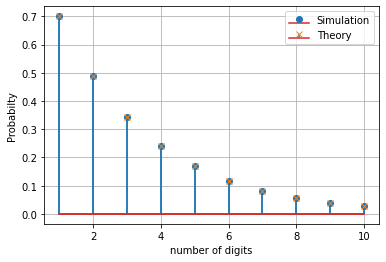
\includegraphics[width=\linewidth]{figs/3.png}
    \caption{Plot  }
    \label{3:}
\end{figure}
\item Three fair cubical dice are thrown simultaneously. The probability that all three dice have the same number of dots on the faces showing up is (up to third decimal place)...........
\solution
Let 
\begin{align}
X_{1},X_{2},X_{3} \in \{1,2,3,4,5,6\}
\end{align}
represent the three dice.

Since, all the three are fair dice, the probability of any dice showing a particular number is given by
\begin{align}
 \pr{X=i} =
    \begin{cases}
      \frac{1}{6} & \text{i=1,2,3,4,5,6}\\
       0 & \text{otherwise}
    \end{cases}       
\end{align}
If all the dice show a particular number i,
\begin{align}
\implies \pr{X_{1} =X_{2}=X_{3}=i}
\end{align}
Since the events are independent, 
\begin{multline}\label{eq1}
  \pr{X_{1} =X_{2}=X_{3}=i}\\
  =  \pr{X_{1}=i}\pr{X_{2}=i}\pr{X_{3}=i}
\end{multline}
where i=1,2,3,4,5,6.\\
There are 6 faces on a cubical dice. Hence, there are six cases in which all the dice show the same number
\begin{align}
 \pr{X_1 =X_2 =X_3}&=\sum^{6}_{i=1} \pr{X_{1} =X_{2}=X_{3}=i}
 \end{align}
 From \eqref{eq1},we have
 \begin{multline}
\pr{X_1 =X_2 =X_3}
\\=\sum^{6}_{i=1}\pr{X_{1}=i}\pr{X_{2}=i}\pr{X_{3}=i}
\end{multline}
\begin{align}
 &=\sum^{6}_{i=1}\brak{\frac{1}{6}}\brak{\frac{1}{6}}\brak{\frac{1}{6}}\\
 &=\frac{1}{36}
\end{align}

\item Candidates were asked to come to an interview with 3 pens each. Black,blue,green and red were the permitted pen colours that the candidate could bring. The probability that a candidate comes with all 3 pens having the same colour is.......

\item The probability of getting a "head" in a single toss of a biased coin is 0.3. The coin is tossed repeatedly till a "head" is obtained. If the tosses are independent, then the probability of getting "head" for the first time in the fifth toss is........
\solution
Let $X\in\mathbb{N}$ represent the number of times the experiment is performed. \\
$X=k$ represents $k-1$ failures were obtained before getting 1 success. $p$ represents the probability of success
\begin{align}
	p_X(k) &=
\begin{cases}
\brak{1-p}^{k-1}\times p & k\in \mathbb{N}\\
0 &  otherwise 
\end{cases}
\label{eq:final_result}
\end{align}
Using \eqref{eq:final_result} we get
\begin{align}
\pr{X=5}&=\brak{1-p}^{k-1}\times p\nonumber\\
&=\brak{0.7}^4\times 0.3=0.07203
\end{align}


\item Given Set A = [2,3,4,5] and Set B = [11,12,13,14,15], two numbers are randomly selected,one from each set. What is probability that the sum of the two numbers equals 16?

\begin{enumerate}
\begin{multicols}{4}
\setlength\itemsep{2em}

\item $
0.20
$
\item $
0.25
$
\item $
0.30
$
\item $
0.33
$

\end{multicols}
\end{enumerate}

\item Consider a dice with the property that the probability of a face with \textit{n} dots showing up is proportional to \textit{n}. The probability of the face with three dots showing up is......

\item \textbf{Step 1.} Flip a coin twice.\\
\textbf{Step 2.} If the outcomes are (TAILS, HEADS) then output Y and stop.\\
\textbf{Step 3.} If the outcomes are either (HEADS, HEADS) or (HEADS, TAILS), then output N and stop.\\
\textbf{Step 4.} If the outcomes are (TAILS, TAILS), then go to Step 1.\\
The probability that the output of the experiment is Y is (upto two decimal places)......


\item Let X and Y denote the sets containing 2 and 20 distinct objects respectively and F denote the set of all possible functions defined from X and Y. Let f be randomly chosen from F. The probability of f being one-to-one is........

\item The probability that a given positive integer lying between 1 and 100 (both inclusive) is NOT divisible by 2,3 or 5 is......
\\
\solution
Let $X \in  \{1,2,...,100\}$ be the random variable representing the outcome for random selection of a number in $\{1,...,100\}$.

Since X has a uniform distribution, the probability mass function (pmf) is represented as 
\begin{align}
    \pr{X  = n} = 
    \begin{cases}
        \frac{1}{100} & 1  \le n \le 100 \\
        0 & otherwise
    \end{cases}
\end{align}
Let A represent the event that the number is divisible by 2.
Let B represent the event that the number is divisible by 3.
Let C represent the event that the number is divisible by 5.

We need to find the probability that the number is not divisible by 2, 3 or 5. Thus we need to find $1 - \pr{A+B+C}$

We know 
\begin{multline}
    \pr{A+B+C} = \pr{A} + \pr{B} + \pr{C} \\- \pr{AB} - \pr{BC} \\- \pr{AC} + \pr{ABC}\label{Shurururururururu}    
\end{multline}

\begin{table}[!ht]
\begin{center}
\begin{tabular}{|c|c|c|}
\hline
Event & Interpretation  & Probability  \\
\hline
A    & n is divisible by 2  & $\cfrac{50}{100}$ \\
B    & n is divisible by 3  & $\cfrac{33}{100}$ \\
C    & n is divisible by 5  & $\cfrac{20}{100}$ \\
AB   & n is divisible by 6  & $\cfrac{16}{100}$ \\
BC   & n is divisible by 15 & $\cfrac{6}{100}$ \\
AC   & n is divisible by 10 & $\cfrac{10}{100}$ \\
ABC  & n is divisible by 30 & $\cfrac{3}{100}$ \\
\hline
\end{tabular}
\end{center}
\caption{}
\label{gate:11}
\end{table}
%
Substituting in \eqref{Shurururururururu}, we get
\begin{multline}
    \pr{A+B+C} = \frac{50}{100} + \frac{33}{100} + \frac{20}{100} \\- \frac{16}{100} - \frac{6}{100} - \frac{10}{100} + \frac{3}{100} 
\end{multline}
Thus, 
\begin{align}
    \pr{A+B+C} = \frac{74}{100}
\end{align}
Thus required probability = 
\begin{align}
    1 - \pr{A+B+C} = \frac{26}{100}
\end{align}


\item P and Q are considering to apply for a job. The probability that P applies for the job is $\dfrac{1}{4}$, the probability that P applies for the job given that Q applies for the job is $\dfrac{1}{2}$, and the probability that Q applies for the job given that P applies for the job is $\dfrac{1}{3}$. Then the probability that P does not apply for the job given that Q does not apply for the job is 

\begin{enumerate}
\begin{multicols}{4}
\setlength\itemsep{2em}

\item $
\dfrac{4}{5}
$

\item $
\dfrac{5}{6}
$

\item $
\dfrac{7}{8}
$

\item $
\dfrac{11}{12}
$

\end{multicols}
\end{enumerate}

\item Two players, A and B, alternately keep rolling a fair dice. The person to get a six first wins the game. Given that player A starts the game, the probability that A wins the game is

\begin{enumerate}
\begin{multicols}{4}
\setlength\itemsep{2em}

\item $
\dfrac{5}{11}
$
\item $
\dfrac{1}{2}
$
\item $
\dfrac{7}{13}
$
\item $
\dfrac{6}{11}
$

\end{multicols}
\end{enumerate}

\item A continuous random variable X has a probability density function $f(x) = e^{-x}, 0<x<\infty$. Then $P(X>1)$ is
\begin{enumerate}
\begin{multicols}{4}
\setlength\itemsep{2em}

\item $0.368$
\item $0.5$
\item $0.632$
\item $1.0$

\end{multicols}
\end{enumerate}

\item A random variable X has probability density function $f(x)$ as given below:\\
$
f(x) =
\begin{cases}
a+bx
&  0<x<1
\\
0
& \text{otherwise}
\end{cases}
$\\
If the expected value $E[X]=\dfrac{2}{3}$, then $Pr[X<0.5]$ is..........

\item Two independent random variables X and Y are uniformly distributed in the interval $[-1,1]$.The probability that max$[X,Y]$ is less than $\dfrac{1}{2}$ is

\begin{enumerate}
\begin{multicols}{4}
\setlength\itemsep{2em}

\item $
\dfrac{3}{4}
$
\item $
\dfrac{9}{16}
$
\item $
\dfrac{1}{4}
$
\item $
\dfrac{2}{3}
$
\end{multicols}
\end{enumerate}

\item The input X to the binary Symmetric Channel (BSC) shown in Fig. \ref{fig:7} is '1' with probability 0.8. The cross-over probability is $\dfrac{1}{7}$. If the received bit Y=0, the conditional probability that '1' was transmitted is........\\


\begin{figure}[!h]
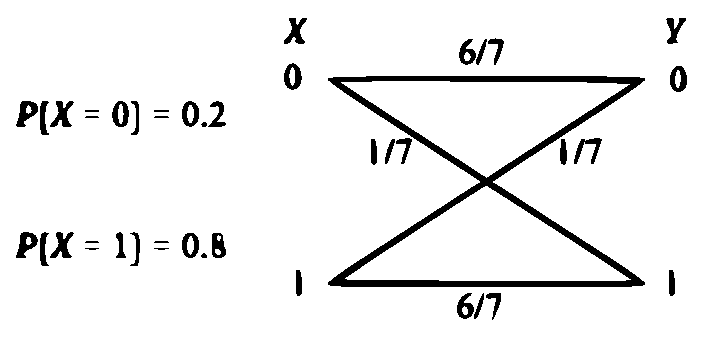
\includegraphics[width=\columnwidth]{./figs/figure7.eps}
\caption{}
\label{fig:7}
\end{figure}


\item A fair coin is tossed till a head appears for the first time. The probability that the number of requried tosses is odd,is
\begin{enumerate}
\begin{multicols}{4}
\setlength\itemsep{2em}
\item $
\dfrac{1}{3}
$
\item $
\dfrac{1}{2}
$
\item $
\dfrac{2}{3}
$
\item $
\dfrac{3}{4}
$
\end{multicols}
\end{enumerate}

\item A box contains 4 white balls and 3 red balls. In succession, two balls are randomly selected and removed from the box. Given that the first removed ball is white, the probability that the second removed ball is red is
\begin{enumerate}
\begin{multicols}{4}
\setlength\itemsep{2em}
\item $
\dfrac{1}{3}
$
\item $
\dfrac{3}{7}
$
\item $
\dfrac{1}{2}
$
\item $
\dfrac{4}{7}
$

\end{multicols}
\end{enumerate}

\item Let X be a random variable with probability density function
$
f(x) = 
\begin{cases}
0.2 & |x|\leqslant1
\\
0.1 & 1\leqslant|x|\leqslant4
\\
0 &  \text{otherwise}.
\end{cases}
$\\
The probability $P(0.5<X,5)$ is..........

\item Consider two identically distributed zero-mean random variables U and V. Let the cumulative distribution functions of U and 2V be F(\textit{x}) and G(\textit{x}) respectively. Then,for all values of \textit{x}
\begin{enumerate}
\begin{multicols}{2}
\setlength\itemsep{2em}
{\small
\item $
F(x)-G(x)\leqslant0
$
\item $
F(x)-G(x)\geqslant0
$
\item $
(F(x)-G(x))\textit{x}\leqslant0
$
\item $
(F(x)-G(x))\textit{x}\geqslant0
$
}
\end{multicols}
\end{enumerate}

%\item Let U and V be two independent and identically distributed random variables such that $
%P(U=+1)=P(U=-1)=\dfrac{1}{2}.
%$
%The entropy H(U+V) in bits is
%
%\begin{enumerate}
%\begin{multicols}{4}
%\setlength\itemsep{2em}
%\item $
%\dfrac{3}{4}
%$
%\item 1
%\item $
%\dfrac{3}{2}
%$
%\item $\log_23
%$

%\end{multicols}
%\end{enumerate}

\item Let U and V be two independent zero mean Gaussian random variables of variances $\dfrac{1}{4}$ and $\dfrac{1}{9}$ respectively. The probability $P(3V\geqslant2U)$ is
\begin{enumerate}
\begin{multicols}{4}
\setlength\itemsep{2em}
\item $
\dfrac{4}{9}
$
\item $
\dfrac{1}{2}
$
\item $
\dfrac{2}{3}
$
\item $
\dfrac{5}{9}
$
\end{multicols}
\end{enumerate}

\item Two independent random variables X and Y are uniformly distributed in the interval $[-1,1]$. The probability that max $[X,Y]$ is less than $\dfrac{1}{2}$ is
\begin{enumerate}
\begin{multicols}{4}
\setlength\itemsep{2em}
\item $
\dfrac{3}{4}
$
\item $
\dfrac{9}{16}
$
\item $
\dfrac{1}{4}
$
\item $
\dfrac{2}{3}
$
\end{multicols}
\end{enumerate}

\item A binary symmetric channel (BSC) has a transition probability of $\dfrac{1}{8}$. If the binary transmit symbol X is such that $P(X=0)=\dfrac{9}{10}$, then the probability of error for an optimum receiver will be
\begin{enumerate}
\begin{multicols}{4}
\setlength\itemsep{2em}
\item $
\dfrac{7}{80}
$
\item $
\dfrac{63}{80}
$
\item $
\dfrac{9}{10}
$
\item $
\dfrac{1}{10}
$
\end{multicols}
\end{enumerate}
\solution

\begin{figure}[h!]
\centering
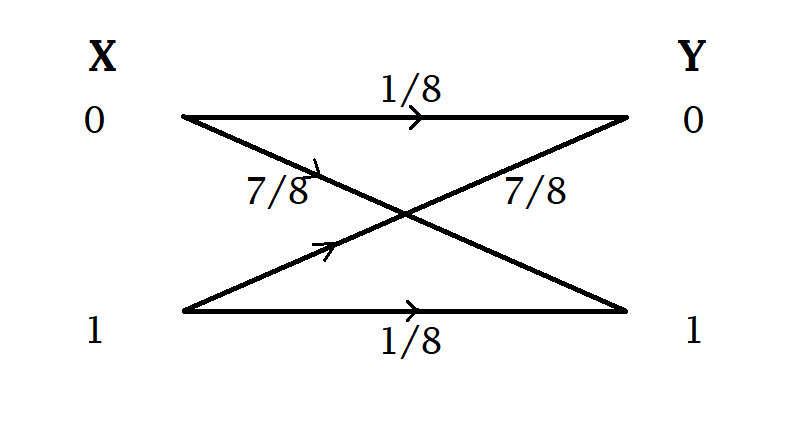
\includegraphics[width=\columnwidth]{solutions/24/Figure.png}
\caption{Binary symmetric channel}
\label{fig:BSC}
\end{figure}

Let random variables, $X \in \{0,1\}$ denote the bit transmitted and $Y \in \{0,1\}$ denote the output bit received.
\\From the given information, 
\begin{align}
    \pr{X=0} = \frac{9}{10}\\
    \pr{X=1} = 1-\pr{X=0} = \frac{1}{10}
\end{align}
Also given, transition probability = $\frac{1}{8}$. Transition probability is the probability with which the bit is transmitted correctly. That gives, 
\begin{align}
    \pr{Y=1|X=1}=\pr{Y=0|X=0}=\frac{1}{8}
\end{align}
\begin{multline}
\text{Probability that the bit is not transmitted correctly}  \\
= 1-\text{transition probability}\\
= 1-\frac{1}{8} = \frac{7}{8}
\end{multline}
That gives,
\begin{align}
    \pr{Y=0|X=1}=\pr{Y=1|X=0}=\frac{7}{8}
\end{align}
Let E denote the event that bit is transmitted incorrectly. Probability of error, $\pr{E}$
\begin{multline}
    \pr{E} = \pr{X=0}\pr{Y=1|X=0}\\ + \pr{X=1}\pr{Y=0|X=1}
\end{multline}
On substituting the values,
\begin{align}
    \pr{E} & = \frac{9}{10}\times\frac{7}{8} + \frac{1}{10}\times\frac{7}{8} \\
    & = \frac{63}{80} + \frac{7}{80}\\
    & = \frac{7}{8}
\end{align}
\rightline{Answer: No option matches}



\item A fair coin is tossed till a head appears for the first time. The probability that the number of requried tosses is odd,is
\begin{enumerate}
\begin{multicols}{4}
\setlength\itemsep{2em}
\item $
\dfrac{1}{3}
$
\item $
\dfrac{1}{2}
$
\item $
\dfrac{2}{3}
$
\item $
\dfrac{3}{4}
$
\end{multicols}
\end{enumerate}

%\item A BPSK scheme operating over an AWGN channel with noise power spectral density of $\dfrac{N_0}{2}$, uses equiprobable signals $
%s_1(t) = {\sqrt{\frac{2E}{T}}} \sin (\omega_ct)
%$ and $
%s_2(t) = {\sqrt{\frac{2E}{T}}} \sin (\omega_ct)
%$
%over the symbol interval $(0,T)$. If the local oscillator in a coherent receiver is ahead in phase by $45\degree$ with respect to the received signal, the probability of error in the resulting system is
%\begin{enumerate}
%\begin{multicols}{4}
%\setlength\itemsep{2em}
%\item $
%Q\bigg(\sqrt{\dfrac{2E}{N_0}}\bigg)
%$
%\item $
%Q\bigg(\sqrt{\dfrac{E}{N_0}}\bigg)
%$
%\item $
%Q\bigg(\sqrt{\dfrac{E}{2N_0}}\bigg)$
%\item $
%Q\bigg(\sqrt{\dfrac{E}{4N_0}}\bigg)$
%
%\end{multicols}
%\end{enumerate}

\item A fair dice is tossed two times. The probability that the second toss result in a value that is higher than the first toss is
\begin{enumerate}
\begin{multicols}{4}
\setlength\itemsep{2em}
\item $
\dfrac{2}{36}
$
\item $
\dfrac{2}{6}
$
\item $
\dfrac{5}{12}
$
\item $
\dfrac{1}{2}
$
\end{multicols}
\end{enumerate}

\item A fair coin is tossed 10 times. What is the probability that ONLY the first two tosses will yield heads?
\begin{enumerate}
\begin{multicols}{2}
\setlength\itemsep{1em}
{\small
\item $
\brak{\frac{1}{2}}^2
$
\item $
{\comb{10}{2}}\brak{\frac{1}{2}}^2
$
\item $
\brak{\frac{1}{2}}^{10}
$
\item $
{\comb{10}{2}}\brak{\frac{1}{2}}^{10}
$
}
\end{multicols}
\end{enumerate}

\item Consider two independent random variables X and Y with identical distributions. The variables X and Y take value 0, 1 and 2 with probabilities $\dfrac{1}{2}$, $\dfrac{1}{4}$ and $\dfrac{1}{4}$ rrespectively. What is the conditional probability $P(X+Y = 2|X-Y =0)$?

\begin{enumerate}
\begin{multicols}{4}
\setlength\itemsep{2em}

\item 0
\item $\dfrac{1}{16}$
\item $\dfrac{1}{6}$
\item 1

\end{multicols}
\end{enumerate}

\item A discrete random variable X takes values from 1 to 5 with probabilities as shown in the table. A student calculates the mean of X as 3.5 and her teacher calculates the variance of X as 1.5. Which of the following statements is true?

\begin{center}
\begin{tabular}{|c|c|c|c|c|c|}\hline

k & 1 & 2 & 3 & 4 & 5\\ \hline
P(X=k) & 0.1 & 0.2 & 0.4 & 0.2 & 0.1\\ \hline
\end{tabular}
\end{center}

\begin{enumerate}
\item Both the student and the teacher are right
\item Both the student and the teacher are wrong
\item The student is wrong but the teacher is right
\item The student is right but the teacher is wrong
\end{enumerate}

%\item A communication channel with AWGN operating at a signal to noise $SNR\gg1$ and bandwidth B has capacity $C_1$. If the SNR is doubled keeping B constant, the resultant capacity $C_2$ is given by
%
%\begin{enumerate}
%\begin{multicols}{4}
%\setlength\itemsep{2em}
%
%\item $
%C_2 \approx 2C_1
%$
%\item $
%C_2 \approx C_1 + B
%$
%\item $
%C_2 \approx C_1 + 2B
%$
%\item $
%C_2 \approx C_1 + 0.3B
%$
%\end{multicols}
%\end{enumerate}

\item If E denotes expectation, the variance of a random variable X is given by
\begin{enumerate}
\begin{multicols}{2}
\setlength\itemsep{2em}
\item $
E[X^2]-E^2[X]
$
\item $
E[X^2]+E^2[X]
$
\item $
E[X^2]
$
\item $
E^2[X]
$
\end{multicols}
\end{enumerate}

\item An examination consists of two papers, Paper 1 and Paper 2. The probability of failing in Paper 1 is 0.3 and that in Paper 2 is 0.2. Given that a student has failed in Paper 2, the probability of failing in Paper 1 is 0.6. The probability  of a student failing in both the papers is:
\begin{enumerate}
\begin{multicols}{4}
\setlength\itemsep{2em}
\item 0.5
\item 0.18
\item 0.12
\item 0.06

\end{multicols}
\end{enumerate}

\item A probability density function is of the form\\
{\centering $p(\textit{x}) = Ke^{-\alpha |x|}, \textit{x}\in(-\infty,\infty)$\\}
The value of K is 

\begin{enumerate}
\begin{multicols}{4}
\setlength\itemsep{2em}

\item 0.5
\item 1
\item $0.5\alpha$
\item $\alpha$

\end{multicols}
\end{enumerate}

\item Consider a binary digital communication system with equally likely 0's and 1's. When binary 0 is transmitted the voltage at the detector input can lie between the level -0.25V and +0.25V with equal probability: when binary 1 is transmitted, the voltage at the detector can have any value between 0 and 1V with equal probability. If the detector has a threshold of 2.0V (i.e., if the received signal is greater than 0.2V, the bit is taken as 1), the average bit error probability is
\begin{enumerate}
\begin{multicols}{4}
\setlength\itemsep{2em}

\item 0.15
\item 0.2
\item 0.05
\item 0.5
\end{multicols}
\end{enumerate}

\item Let X and Y be two statistically independent random variables uniformly distributed in the range $(-1,1)$ and $(-2,1)$ respectively. Let $Z = X+Y$, then the probability that $[Z\leqslant-2]$ is
\begin{enumerate}
\begin{multicols}{4}
\setlength\itemsep{2em}
\item zero
\item $\dfrac{1}{6}$
\item $\dfrac{1}{3}$
\item $\dfrac{1}{12}$
\end{multicols}
\end{enumerate}

\item Let X be the Gaussian random variable obtained by sampling the process at $t=t_i$ and let 
\begin{equation*}
Q(\alpha)={\int_{\alpha}^{\infty}}\dfrac{1}{\sqrt{2\pi}}e^{\frac{-y^2}{2}}dy
\end{equation*}
%
The probability that $[\textit{X}\leqslant1]$ is \dots
%

%\begin{enumerate}
%\begin{multicols}{2}
%\setlength\itemsep{1em}
%\item $
%1-Q(0.5)
%$
%\item $Q(0.5)$
%\item $Q\brak{\frac{1}{2\sqrt{2}}}
%$
%\item $
%1-Q\brak{\frac{1}{2\sqrt{2}}}
%$
%\end{multicols}
%\end{enumerate} 
%


\item Let Y and Z be the random variables obtained by sampling $X(t)$ at $t=2$ and $t=4$ respectively. Let W = Y-Z. The variance of W is
\begin{enumerate}
\begin{multicols}{4}
\setlength\itemsep{2em}
\item 13.36
\item 9.36
\item 2.64
\item 8.00

\end{multicols}
\end{enumerate}

%\item Let $(X_1,X_2)$ be independent random variables. $X_1$ has mean 0 and variance 1, while $X_2$ has mean 1 and variance 4. The mutual information I $(X_1;X_2)$ between $X_1$ and $X_2$ in bits is.......

\item Let the random variable X represent the number of times a fair coin needs to be tossed till two consecutive heads appear for the first time. The expectation of X is......

\item Let $X\in[0,1]$ and $Y\in[0,1]$ be two independent binary random variables. If $P(X=0) = p$ and $P(Y=0) = q$, then $P(X+Y\geqslant1)$ is equal to

\begin{enumerate}
\begin{multicols}{2}
\setlength\itemsep{1em}
{\small
\item $
pq + (1-p)(1-q)
$
\item pq
\item $p(1-q)$
\item $1-pq$
}
\end{multicols}
\end{enumerate}

\item Suppose A and B are two independent events with probabilities $P(A)\neq 0$ and $P(B)\neq0$. Let $\widetilde A$ and $\widetilde B$ be their complements. Which one of the following statements is FALSE?

\begin{enumerate}
\begin{multicols}{2}
\setlength\itemsep{1em}
{\scriptsize
\item $
P(A \cap B) = P(A)P(B)
$
\item $
P(A|B) = P(A)
$
\item $
P(A \cup B) = P(A)+P(B)
$
\item $
P(\widetilde A \cap \widetilde B) = P(\widetilde A)P(\widetilde B)
$
}
\end{multicols}
\end{enumerate}

\item A digital communication system uses a repetition code for channel encoding/decoding. During transmission, each bit is repeated three times(0 is transmitted as 000, and 1 is transmitted as 111). It is assumed that the source puts out symbols independently and with equal probability. The decoder operates as follows: In a block of three received bits, if the number of zeros exceeds the number of ones, the decoder decides in favour of a 0, and if the number of ones exceeds the number of zeros, the decoder decides in favour of a 1. Assuming a binary symmetric channel with crossover probability p = 0.1, the average probability of error is ........

\item Two random variables X and Y are distributed according to\\
{\centering $
f_{x,y}(x,y) = 
\begin{cases}
 (x+y) & 0 \leqslant x \leqslant 1   0 \leqslant y \leqslant 1 \\
 0 & \text{otherwise}.
 \end{cases}
 $ \\}
The probability $P(X+Y \leqslant 1)$ is .......

%\item A binary communication system makes use of the symbols "zero" and "one". There are channel errors. Consider the following events:
%\begin{itemize}
%\item $x_0$:a "zero" is transmitted
%\item $x_1$:a "one" is transmitted
%\item $y_0$:a "zero" is received
%\item $y_1$:a "one" is received
%\end{itemize}
%%
%The following probabilities are given: $P(x_0) = \frac{1}{2}$, $P(y_0|x_0)= \frac{3}{4}$, and $P(y_0|x_1)= \frac{1}{2}$. The information in bits that you obtain when you learn which symbol has been received (while you know that a "zero" has been transmitted) is .........

\item Let X be a zero mean unit variance Gaussian random variable. $E[|X|]$ is equal to .........

\item If calls arrive at a telephone exchange such that the time of arrival of any call is independent of the time of arrival of earlier or future calls, the probability distribution function of the toatl number of calls in a fixed time interval will be

\begin{enumerate}
\begin{multicols}{2}
\setlength\itemsep{2em}

\item Poisson
\item Gaussian
\item Exponential
\item Gamma

\end{multicols}
\end{enumerate}

\item Consider a communication scheme where the binary valued signal X satisfies $P\{X = +1\} = 0.75$ and $P\{X = -1\} = 0.25$. The received signal $Y = X+Z$, where Z is a Gaussian random variable with zero mean and variance $\sigma^2$. The received signal Y is fed to the threshold detector. The output of the threshold detector $\hat X$ is:\\
{\centering $
{\hat X}= 
\begin{cases} 
+1 & Y> \tau \\
-1 & Y \leqslant \tau 
\end{cases}
$\\}
To achieve minimum probability of error $P\{\hat X \neq X\}$, the threshols $ \tau$ should be

\begin{enumerate}
\begin{multicols}{2}
\setlength\itemsep{2em}

\item strictly positive
\item zero
\item strictly negative
\item strictly positive, zero or strictly negative depending on the nonzero value of $\sigma ^2$

\end{multicols}
\end{enumerate}

\item Consider a discrete-time channel $Y = X+Z$, where the additive noise Z is signal-dependent. In particular, given the transmitted symbol $X \in \{-a,+a\}$ at any instant, the noise sample Z is chosen independently from a Gaussian distribution with mean $\beta X$ and unit variance. Assume a threshold detector with zero threshold at the receiver.\\
When $\beta = 0$, the BER was found to be $Q(a) = 1 \times {10^-8}$.\\
$$
\bigg(Q(v)= \dfrac{1}{\sqrt{2 \pi}} \int_{v}^{\infty} e^{\frac{-u^2}{2}}du$$, and for $v>1$, use $Q(v) \approx e^{\frac{-v^2}{2}} \bigg)$ \\
When $\beta = -0.3$, the BER is closet to

\begin{enumerate}
\begin{multicols}{2}
\setlength\itemsep{2em}

\item $10^-7$
\item $10^-6$
\item $10^-4$
\item $10^-2$

\end{multicols}
\end{enumerate}

\item Consider the random process\\
$ X(t) = U+Vt$,\\
where U is a zero-mean Gaussian random variable and V is a random variable distributed between 0 and 2. Assume that U and V are statistically independent. The mean value of the random  process at t=2 is........
%
\solution
Here U is a gaussian random variable of mean 0 and Let us consider V is uniformly distributed random variable in $(0,2)$.
\begin{table}[h]
\centering
\begin{tabular}{|c|c|c|c|}
\hline
   Random Variable             & U & V & X(t)  \\ \hline
Expected Value & 0 & 1 & t\\ \hline
\end{tabular}
\caption{Random Variables and Expected Values}
\label{tab:expected values}
\end{table}

From Table \ref{tab:expected values} we can deduce that,
\begin{align}
    E\sbrak{X(t)}&=E\sbrak{U+Vt}\\
    E\sbrak{X(t)}&=E\sbrak{U}+tE\sbrak{V}\\
    E\sbrak{X(t)}&=0+t\\
    E\sbrak{X(t)}&=t\\
    E\sbrak{X(2)}&=2
\end{align}
 $ \therefore$ mean of random process X(t) at 2 is 2.


\item Consider the Z-channel given in Fig. \ref{fig:1}. The input is 0 or 1 with equal probability.
\begin{figure}[!h]
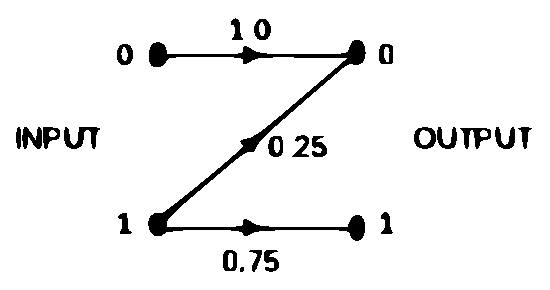
\includegraphics[width=\columnwidth]{./figs/figure1.eps}
\caption{}
\label{fig:1}
\end{figure}



If the output is 0, the probability that the input is also 0 equals......

\item If P and Q are two random events, then the following is TRUE:

\begin{enumerate}

\item Independence of P and Q implies that $\Pr{P \cap Q} = 0$
\item $\Pr(P \cup Q)\geqslant \Pr(P)+\Pr(Q)$
\item If P and Q are mutually exclusive, then they must be independent
\item $\Pr(P \cap Q)\leqslant \Pr(P)$

\end{enumerate}

\item A fair coin is tossed three times in succession. If the first toss produces a head, then the probability of getting exactly two heads in three tosses is:

\begin{enumerate}
\begin{multicols}{2}
\setlength\itemsep{1em}

\item $\frac{1}{8}$
\item $\frac{1}{2}$
\item $\frac{3}{8}$
\item $\frac{3}{4}$

\end{multicols}
\end{enumerate}

\item The probability density function (PDF) of a random variable X is as shown in Fig. \ref{fig:2}.
\begin{figure}[!h]
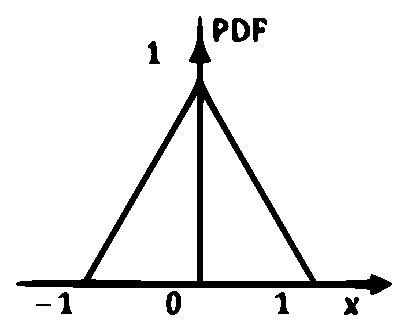
\includegraphics[width=\columnwidth]{./figs/figure2.eps}
\caption{}
\label{fig:2}
\end{figure}

The corresponding cumulative distribution function (CDF) has the form\\

\begin{enumerate}
\begin{multicols}{2}
\setlength\itemsep{4em}

\item Fig. \ref{fig:3}

%\includegraphics{figure3.eps}
\item Fig. \ref{fig:4}

%\includegraphics{figure4.eps}
\item Fig. \ref{fig:5}

% \includegraphics{figure5.eps}
\item Fig. \ref{fig:6}


%\includegraphics{figure6.eps}

\end{multicols}
\end{enumerate}
\begin{figure}[!h]
\includegraphics[width=\columnwidth]{./figs/figure3.eps}
\caption{}
\label{fig:3}
\end{figure}
\begin{figure}[!h]
\includegraphics[width=\columnwidth]{./figs/figure4.eps}
\caption{}
\label{fig:4}
\end{figure}
\begin{figure}[!h]
\includegraphics[width=\columnwidth]{./figs/figure5.eps}
\caption{}
\label{fig:5}
\end{figure}

\begin{figure}[!h]
\includegraphics[width=\columnwidth]{./figs/figure6.eps}
\caption{}
\label{fig:6}
\end{figure}



%\item Consider a binary, digital communication system which uses pulses g(t) and -g(t) for transmitting bits over an AWGN channel. If the receiver uses a matched filter, which one of the following pulses will give the minimum probability of bit error?\\
%
%\begin{enumerate}
%\begin{multicols}{2}
%\setlength\itemsep{4em}
%
%
%\item Fig. \ref{fig:8}
%\item Fig. \ref{fig:9}
%\item Fig. \ref{fig:10}
%\item Fig. \ref{fig:11}
%
%\end{multicols}
%\end{enumerate}
%\begin{figure}[!h]
%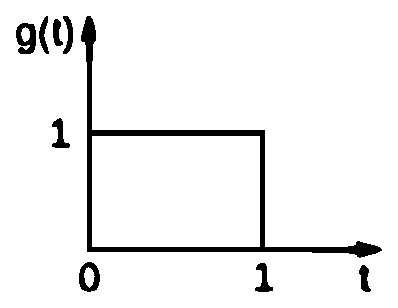
\includegraphics[width=\columnwidth]{./figs/figure8.eps}
%\caption{}
%\label{fig:8}
%\end{figure}
%\begin{figure}[!h]
%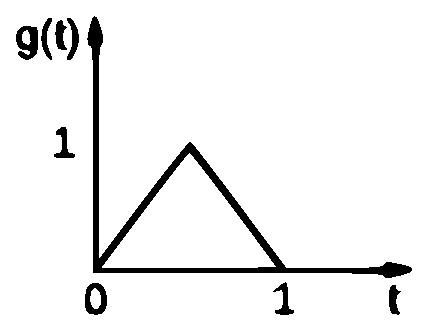
\includegraphics[width=\columnwidth]{./figs/figure9.eps}
%\caption{}
%\label{fig:9}
%\end{figure}
%\begin{figure}[!h]
%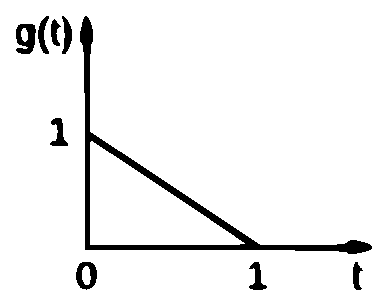
\includegraphics[width=\columnwidth]{./figs/figure10.eps}
%\caption{}
%\label{fig:10}
%\end{figure}
%\begin{figure}[!h]
%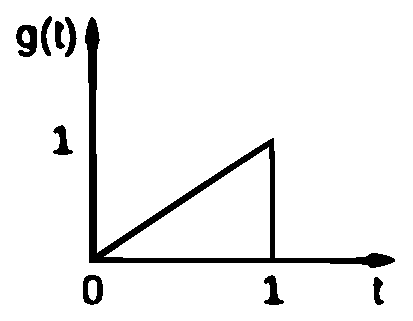
\includegraphics[width=\columnwidth]{./figs/figure11.eps}
%\caption{}
%\label{fig:11}
%\end{figure}


\item The distribution function $f_x(x)$ of a random variable X is shown in Fig. \ref{fig:12}. The probability that X=1 is
%
\begin{figure}[!h]
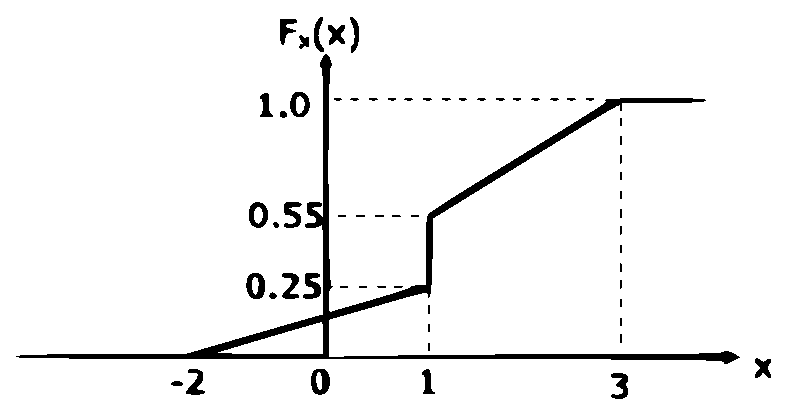
\includegraphics[width=\columnwidth]{./figs/figure12.eps}
\caption{}
\label{fig:12}
\end{figure}


\begin{enumerate}
\begin{multicols}{2}
\setlength\itemsep{1em}

\item Zero
\item 0.25
\item 0.55
\item 0.30

\end{multicols}
\end{enumerate}


%\begin{center}
%\centering\underline{\textbf{Common Data for the following two Questions :}}
%\end{center}

%\item Let $X$ be a random variable with probability density function $f \in \{f_0,f_1\},$ where 
%
%$ 
%f_0(x)=
%\begin{cases}
%2x & 0<x<1 \\
%0 & \text{otherwise}
%\end{cases}
%$ \\
%
%$ 
%f_1(x)=
%\begin{cases}
%3x^2 &  0<x<1 \\
%0 & \text{otherwise}
%\end{cases}
%$\\
%
%For testing the null hypothesis $H_0:f \equiv f_0$ against the alternative hypothesis $H_1:f \equiv f_1$ at level of significance $\alpha = 0.19$, the power of the most powerful test is
%
%\begin{enumerate}
%\begin{multicols}{2}
%\setlength\itemsep{2em}
%
%\item $ 0.729$
%\item $ 0.271$
%\item $ 0.615$
%\item $ 0.385$
%
%\end{multicols}
%\end{enumerate}
%

%\item The variance of the random variable $X$ is
%
%\begin{enumerate}
%\begin{multicols}{2}
%\setlength\itemsep{2em}
%
%\item $ \frac{1}{12}$
%\item $ \frac{1}{4}$
%\item $ \frac{7}{12}$
%\item $ \frac{5}{12}$
%
%\end{multicols}
%\end{enumerate}
%
%
%\item The covariance between the random variables $X$ and $Y$ is
%
%\begin{enumerate}
%\begin{multicols}{2}
%\setlength\itemsep{2em}
%
%\item $ \frac{1}{3}$\\
%\item $ \frac{1}{4}$\\
%\item $ \frac{1}{6}$\\
%\item $ \frac{1}{12}$\\
%
%\end{multicols}
%\end{enumerate}

\item Let the probability density function of a random variable $X$ be 
\begin{center}
$ 
f(x)=
\begin{cases}
x & 0\leq\ x< \frac{1}{2}\\
c(2x-1)^2 &  \frac{1}{2}<x\leq\ 1\\
0 & \text{otherwise}.
\end{cases}
$\\ 
\end{center}


Then,the value of $c$ is equal to \underline{\hspace{3cm}}
\\

\item Suppose $X$ and $Y$ are two random variables such that $aX + bY$ is a normal random variable for all $a,b \in \mathbb{R}$. Consider the following statements P,Q,R and S:


 (P): $X$ is a standard normal random variable.\\
 (Q): The conditional distribution of $X$ given $Y$ is normal.\\
 (R): The conditional distribution of $X$ given $X$ + $Y$ is normal.\\
 (S): $X$ - $Y$ has mean $0$.\\

Which of the above statements ALWAYS hold TRUE?
\begin{enumerate}
\begin{multicols}{2}
\setlength\itemsep{2em}

\item both P and Q
\item both Q and R
\item both Q and S
\item both P and S

\end{multicols}
\end{enumerate}

 
\item Let $X$ be a random variable with the following cumulative distribution function: 

\begin{center}
$ 
F(x)=
\begin{cases}
0 & x<0 \\
x^2 & 0\leq\ x <\frac{1}{2}\\
\frac{3}{4} & \frac{1}{2}\leq\ x<1\\
1 & x\geq\ 1.
\end{cases}
$\\ 

\end{center}
Then $P\brak{\frac{1}{4}<X<1}$ is equal to \underline{\hspace{3cm}}
\\
 


\item Let $X_1$ be an exponential random variable with mean 1 and $X_2$ a gamma random variable with mean 2 and variance 2. If $X_1$ and $X_2$ are independently distributed,then $P(X_1<X_2)$ is equal to \underline{\hspace{3cm}}
\\

\begin{center}
\centering\underline{\textbf{Common Data for the next two Questions :}}
\end{center}


Let $X$ and $Y$ be jointly distributed random variables such that the conditional distribution of $Y$, given $X$ =$x$, is uniform on the interval $(x-1,x+1)$. Suppose $E(X)=1$ and $Var(X)=\frac{5}{3}$.
\\
\item The mean of the random variable $Y$ is 
\\
\begin{enumerate}
\begin{multicols}{2}
\setlength\itemsep{2em}

\item $ \frac{1}{2}$\\
\item $1$\\
\item $ \frac{3}{2}$\\
\item $2$

\end{multicols}
\end{enumerate}

\item The variance of the random variable $Y$ is 
\\
\begin{enumerate}
\begin{multicols}{2}
\setlength\itemsep{2em}

\item $ \frac{1}{2}$\\
\item $ \frac{2}{3}$\\
\item $1$\\
\item $2$

\end{multicols}
\end{enumerate}


\item Let the random variable $X$ have the distribution function: 
\begin{center}
$ 
F(x)=
\begin{cases}
0 &  \ x<0 \\
\frac{x}{2} &  \ 0\leq\ x <1 \\
\frac{3}{5} &  \ 1\leq\ x<2\\
\frac{1}{2}+\frac{x}{8} &  \ 2\leq\ x<3\\
1 &  \ x\geq\ 3.
\end{cases}
$\\ 
\end{center}

Then $P\brak{2 \leq\ X<4}$ is equal to \underline{\hspace{3cm}}
 \\

\item Let $X$ be a random variable having the distribution function: 
\begin{center}
$ 
F(x)=
\begin{cases}
0 &  \ x<0 \\
\frac{1}{4} &  \ 0\leq\ x <1 \\
\frac{1}{3} &  \ 1\leq\ x<2\\
\frac{1}{2} &  \ 2\leq\ x<\frac{11}{3}\\
1 &  \ x\geq\ \frac{11}{3}.
\end{cases}
$\\ 
\end{center}

Then $E(X)$ is equal to \underline{\hspace{3cm}}
\\
\item Let $X$ and $Y$ be two random variables having the joint probability density function

\begin{center}
$ 
f(x,y)=
\begin{cases}
2 &  \ 0<x<y<1 \\
0 & \text{otherwise}.
\end{cases}
$\\ 
\end{center}

Then the conditional probability $P \brak{X \leq\ \frac{2}{3} | Y=\frac{3}{4}}$ is equal to \underline{\hspace{3cm}}

\begin{enumerate}
\begin{multicols}{4}
\setlength\itemsep{2em}

\item $
\frac{5}{9}
$
\item $
\frac{2}{3}
$
\item $
\frac{7}{9}
$
\item $
\frac{8}{9}
$


\end{multicols}
\end{enumerate}

\item Let $\Omega= (0,1]$ be the sample space and let $P(\cdot)$ be a probability function defined by 

\begin{center}
$ 
P((0,x])=
\begin{cases}
\frac{x}{2} &  \ 0 \leq\ x< \frac{1}{2} \\
x &  \  \frac{1}{2} \leq\ x \leq\ 1.
\end{cases}
$\\ 
\end{center}

Then $P\brak{\lbrace\frac{1}{2}\rbrace}$ is equal to \underline{\hspace{3cm}}
\\

\item Suppose the random variable $U$ has uniform distribution on $[0,1]$ and $X= -2\log U$. The density of $X$ is

\begin{enumerate}

\item $ 
f(x)=
\begin{cases}
e^{-x} &  \ x>0\\
0 & \text{otherwise}.
\end{cases}
$\\ 

\item $ 
f(x)=
\begin{cases}
2e^{-2x} & \ x>0\\
0 & \text{otherwise}.
\end{cases}
$\\ 

\item $ 
f(x)=
\begin{cases}
\frac{1}{2}e^{-\frac{x}{2}} &  \ x>0\\
0 & \text{otherwise}.
\end{cases}
$\\ 

\item $ 
f(x)=
\begin{cases}
\frac{1}{2} &  \ x \in [0,2]\\
0 & \text{otherwise}.
\end{cases}
$\\ 



\end{enumerate}


\item Suppose $X$ is a real-valued random variable.Which of the following values \textbf{CANNOT} be attained by $E[X]$ and $E[X^2]$, respectively?


\begin{enumerate}
\begin{multicols}{2}
\setlength\itemsep{2em}

\item $
0 \ and \ 1
$
\item $
2  \ and \ 3
$
\item $
\frac{1}{2} \ and \ \frac{1}{3}
$
\item $
2 \ and \ 5
$

\end{multicols}
\end{enumerate}

\item Let $X_n$ denote the sum of points obtained when n fair dice are rolled together. The expectation and variance of $X_n$ are

\begin{enumerate}
\begin{multicols}{2}
\setlength\itemsep{1em}
{\scriptsize
\item ${\dfrac{7}{2}}n$ and ${\dfrac{35}{12}}n^2$ respectively.
\item ${\dfrac{7}{2}}n$ and ${\dfrac{35}{12}}n$ respectively.
\item $ \bigg (\dfrac{7}{2} \bigg )^n$ and $ \bigg (\dfrac{35}{12} \bigg )^n$ respectively.
\item None of the above
}
\end{multicols}
\end{enumerate}

\item Let X and Y be jointly distributed random variables having the joint probability density function \\
$
f(x,y) = 
\begin{cases} 
\frac{1}{\pi} 
&  x^2+y^2 \leqslant 1 \\
0 & \text{otherwise}
\end{cases}
$ \\
Then $P(Y>max(X,-X))=$

\begin{enumerate}
\begin{multicols}{2}
\setlength\itemsep{2em}

\item $\dfrac{1}{2}$
\item $\dfrac{1}{3}$
\item $\dfrac{1}{4}$
\item $\dfrac{1}{6}$

\end{multicols}
\end{enumerate}

\item Consider two identical boxes $B_1$ and $B_2$, where the box $B(i=1,2)$ contains $i+2$ red and $5-i-1$ white balls. A fair die is cast. Let the number of dots shown on the top face of the die be N. If N is even or 5, then two balls are drawn with replacement from the box $B_1$, otherwise, two balls are drawn with replacement from the box $B_2$. The probability that the two drawn balls are of different colours is

\begin{enumerate}
\begin{multicols}{2}
\setlength\itemsep{2em}

\item $\dfrac{7}{25}$
\item $\dfrac{9}{25}$
\item $\dfrac{12}{25}$
\item $\dfrac{16}{25}$

\end{multicols}
\end{enumerate}

\begin{center}
\centering\underline{\textbf{Common Data for the next two Questions :}}
\end{center}

Let X and Y be random variables having the joining probability density function \\
$
f(x,y)=
\begin{cases}
{\dfrac{1}{\sqrt{2 \pi y}}}e^{\frac{-1}{2y}(x-y)^2}
& -\infty < x < \infty,\\  
&  0 < y < 1
\\
0 & \text{otherwise}
\end{cases}
$ \\

\item The variance of the random variable X is 

\begin{enumerate}
\begin{multicols}{2}
\setlength\itemsep{2em}

\item $\dfrac{1}{12}$
\item $\dfrac{1}{4}$
\item $\dfrac{7}{12}$
\item $\dfrac{5}{12}$

\end{multicols}
\end{enumerate}

\item The covariance between the random variables X and Y

\begin{enumerate}
\begin{multicols}{2}
\setlength\itemsep{2em}

\item $\dfrac{1}{3}$
\item $\dfrac{1}{4}$
\item $\dfrac{1}{6}$
\item $\dfrac{1}{12}$

\end{multicols}
\end{enumerate}


\begin{center}
\centering\underline{\textbf{Common Data for the next two  Questions :}}
\end{center}

Let X and Y be continuous random variables with the joint probability density function \\

$
f(x,y)=
\begin{cases}
a{e^{-2y}}
& 0 <x<y< \infty \\
0 & \text{otherwise}
\end{cases}
$

\item The value of a is

\begin{enumerate}
\begin{multicols}{2}
\setlength\itemsep{2em}

\item 4
\item 2
\item 1
\item 0.5

\end{multicols}
\end{enumerate}

\item The value of $E(X|Y=2)$ is

\begin{enumerate}
\begin{multicols}{2}
\setlength\itemsep{2em}

\item 4
\item 3
\item 2
\item 1
\end{multicols}
\end{enumerate}

\item Let X and Y be two random variables having the joint probability density function \\

$
f(x,y)=
\begin{cases}
2 &  0<x<y<1 \\
0 & \text{otherwise}
\end{cases}
$ \\
Then the conditional probability $P(X \leqslant {\frac{2}{3}}| Y={\frac{3}{4}})$ is equal to

\begin{enumerate}
\begin{multicols}{2}
\setlength\itemsep{2em}

\item $\dfrac{5}{9}$
\item $\dfrac{2}{3}$
\item $\dfrac{7}{9}$
\item $\dfrac{8}{9}$
\end{multicols}
\end{enumerate}

\item Let $\Omega = (0,1]$ be the sample space and let $P(.)$ be a probability function defined by \\
$
P((0,x])=
\begin{cases}
\frac{x}{2} 
&  0 \leqslant x < \frac{1}{2} \\
x &  \frac{1}{2} \leqslant x \leqslant 1
\end{cases}
$ \\
Then $P \bigg ( \{ \frac{1}{2} \} \bigg )$ is equal to.......

\item Let X be a random variable with the following cumulative distribution function: \\

$
F(x)= 
\begin{cases}
0 & x<0 \\
x^2 & 0 \leqslant x < \frac{1}{2} \\
\frac{3}{4} & \frac{1}{2} \leqslant x < 1 \\
1 & x \geqslant 1
\end{cases}
$ \\

Then $P({\frac{1}{4}}<x<1)$ is equal to........

\item Let $X_1$ be an exponential random variable with mean 1 and $X_2$ a gamma random variable with mean 2 and variance 2. If $X_1$ and $X_2$ are independently distributed, then $P(X_1<X_2)$ is equal to.....

\begin{center}
\centering\underline{\textbf{Common Data for the next two Questions :}}
\end{center}

Let X and Y be two continuous random variables with the joint probability density function \\
$
f(x,y)= 
\begin{cases}
2 & 0<x+y<1, x>0, y>0 \\
0 & \text{elsewhere}.
\end{cases}
$

\item $P(X+Y<\frac{1}{2})$ is

\begin{enumerate}
\begin{multicols}{2}
\setlength\itemsep{2em}

\item $\dfrac{1}{4}$
\item $\dfrac{1}{2}$
\item $\dfrac{3}{4}$
\item 1
\end{multicols}
\end{enumerate}

\item $E(X|Y=\frac{1}{2})$

\begin{enumerate}
\begin{multicols}{2}
\setlength\itemsep{2em}

\item $\dfrac{1}{4}$
\item $\dfrac{1}{2}$
\item 1
\item 2
\end{multicols}
\end{enumerate}

\item If a random variable X assumes only positive integral values, with the probability \\
$
P(X=x) = \frac{2}{3}(\frac{1}{3})^{x-1}$, $x=1,2,3,...,$ \\

then $E(X)$ is

\begin{enumerate}
\begin{multicols}{2}
\setlength\itemsep{2em}

\item $\dfrac{2}{9}$
\item $\dfrac{2}{3}$
\item 1
\item $\dfrac{3}{2}$

\end{multicols}
\end{enumerate}


\item The joint probability density function of two random variables X and Y is given as \\
$
f(x,y)=
\begin{cases}
\dfrac{6}{5}(x+y^2)
& 0 \leqslant x \leqslant 1  0 \leqslant x \leqslant 1 \\
0 & \text{elsewhere}
\end{cases}
$\\
$E(X)$ and $E(Y)$ are, respectively,

\begin{enumerate}
\begin{multicols}{2}
\setlength\itemsep{2em}

\item $\dfrac{2}{5}$ and $\dfrac{3}{5}$
\item $\dfrac{3}{5}$ and $\dfrac{3}{5}$
\item $\dfrac{3}{5}$ and $\dfrac{6}{5}$
\item $\dfrac{4}{5}$ and $\dfrac{6}{5}$
\end{multicols}
\end{enumerate}

\item Suppose the random variable U has uniform distribution on $[0,1]$ and $X= -2 \log U$. The density of X is \\

\begin{enumerate}
\setlength\itemsep{2em}

\item $
f(x)=
\begin{cases}
e^{-x} &  x>0\\
0 & \text{otherwise}
\end{cases}
$

\item $
f(x)=
\begin{cases}
2e^{-2x} &  x>0 \\
0 & \text{otherwise}
\end{cases}
$

\item $
f(x)=
\begin{cases}
\dfrac{1}{2}e^-{\frac{x}{2}} &  x>0 \\
0 & \text{otherwise}
\end{cases}
$

\item $
f(x)=
\begin{cases}
\dfrac{1}{2} &  x \in [0,2] \\
0 & \text{otherwise}
\end{cases}
$

\end{enumerate}

\item Suppose X is a real-valued random variable. Which of the following values CANNOT be attained by $E[X]$ and $E[X^2]$, respectively?

\begin{enumerate}
\begin{multicols}{2}
\setlength\itemsep{2em}

\item 0 and 1
\item 2 and 3
\item $\dfrac{1}{2}$ and $\dfrac{1}{3}$
\item 2 and 5
\end{multicols}
\end{enumerate}

\item Probability density function $p(x)$ of a random variable x is as shown below. The value of $\alpha$ is 

\begin{figure}[!h]
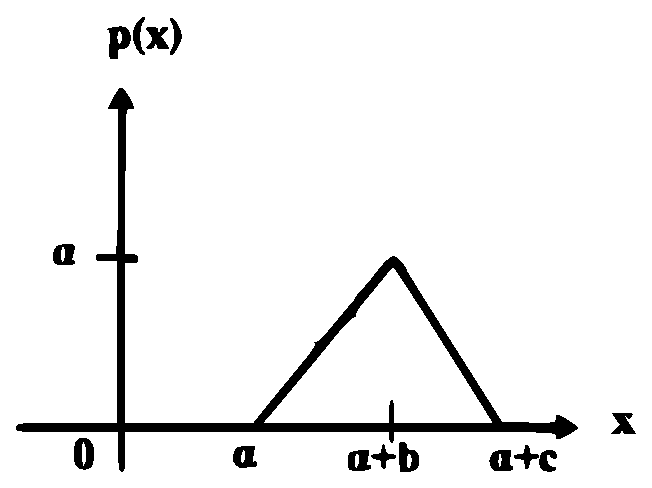
\includegraphics[width=\columnwidth]{./figs/figure13.eps}
\caption{}
\label{fig:13}
\end{figure}


\begin{enumerate}
\begin{multicols}{2}
\setlength\itemsep{2em}

\item $\dfrac{2}{c}$
\item $\dfrac{1}{c}$
\item $\dfrac{2}{(b+c)}$
\item $\dfrac{1}{(b+c)}$

\end{multicols}
\end{enumerate}

\item A player throws a ball at a basket kept at a distance. The probability that the ball falls into the basket in a single attempt is 0.1. The player attempts to throw the ball twice. Considering each attempt to be independent, the probability that this player puts the ball into the basket only in the second attempt is.........
\\
\solution
Let $X\in\mathbb{N}$ represent the number of times the experiment is performed. \\
$X=k$ represents $k-1$ failures were obtained before getting 1 success. $p$ represents the probability of success
\begin{align}
	p_X(k) &=
\begin{cases}
\brak{1-p}^{k-1}\times p & k\in \mathbb{N}\\
0 &  otherwise 
\end{cases}
\label{2020:eq:final_result}
\end{align}
Using \eqref{2020:eq:final_result} we get
\begin{align}
\pr{X=2}&=\brak{1-p}^{k-1}\times p\nonumber\\
&=\brak{0.9}\times 0.1=0.09
\end{align}
\item A screening test is carried out to detect a certain disease. It is found that $12\%$ of the positive
reports and $15\%$ of the negative reports are incorrect. Assuming that the probability of a
person getting positive report is 0.01, the probability that a person tested gets an incorrect
report is \dots
\\
\solution
Let $X \in \{0,1\}$ represent the random variable, where 0 represents the case where a person gets a positive report while 1 represents the case where a person gets a negative report. From the question, 
\begin{align}
    \Pr{(X=0)} = 0.01
    \\\Pr{(X=0)} + \Pr{(X=1)} = 1
    \\\Pr{(X=1)} = 1 - 0.01 = 0.99
\end{align}
Let $Y \in \{0,1\}$ represent the random variable, where 0 represents a correct report whereas 1 represents an incorrect report.

\begin{align}
    \Pr{(Y=1 | X=0)} = 12\% = 0.12
    \\\Pr{(Y=1 | X=1)} = 15\% = 0.15
\end{align}
Then, from total probability theorem,
\begin{multline}
    \Pr{(Y=1)} = \Pr{(Y=1, X=0)} 
    \\+ \Pr{(Y=1, X=1)}
\end{multline}
Using Bayes theorem,
\begin{multline}
    \Pr{(Y=1)} = \Pr{(Y=1 | X=0)} \times \Pr{(X=0)}
    \\ + \Pr{(Y=1 | X=1)} \times \Pr{(X=1)}
\end{multline}
    
\begin{align}
    \Pr{(Y=1)} = & 0.12 \times 0.01 + 0.15 \times 0.99
    \\ = & 0.0012 + 0.1485
    \\ = & 0.1497    
\end{align}
%
\item Shaquille O’ Neal is a 60\% career free throw shooter, meaning that he successfully makes 60 free throws out of 100 attempts on average. What is the probability that he will successfully make exactly 6 free throws in 10 attempts?
\begin{enumerate} [label={\Alph*)}]
\item 0.2508
\item 0.2816
\item 0.2934
\item 0.6000
\end{enumerate}
%
\solution
Let 
\begin{align}
X_{i}\in \{0,1\}
\end{align}
represent the $i^{th}$ free throw, where 1 represents a successful free throw attempt and 0 represents an unsuccessful attempt.
Let
\begin{align}
X=\sum_{i=1}^{n} X_{i}   
\end{align}
where n is the total number of free throws. Then, X has a binomial distribution with
\begin{align}
\pr {X=k}=\comb{n}{k} p^{k} q^{n-k}
\end{align}
Where,
\begin{align}
  &p=\frac{6}{10}\\
  &q=1-p=\frac{4}{10}\\
  &n=10
\end{align}
from the given information. Then,
\begin{align}
\pr{X=6}&=\comb{10}{6}\brak{\frac{6}{10}}^{6}\brak{\frac{4}{10}}^{4}
\end{align}
On simplifying we get,
\begin{align}
\pr{X=6}&=0.2508
\end{align}
Therefore, the probability that he will successfully make exactly 6 free throws in 10 attempts is 0.2508 and hence option (A) is correct.
%
\end{enumerate}
\end{document}
